\documentclass[11pt]{article}
\usepackage[utf8]{inputenc}
\usepackage[spanish,es-nodecimaldot]{babel}
\usepackage[a4paper,margin=2.4cm]{geometry}
\usepackage{amsmath,booktabs,graphicx,siunitx,url}

\title{\textbf{Test 5: Sensibilidad a malla, condiciones de borde y evidencia de verificación}}
\author{Herramientas Computacionales para Ingeniería II --- USACH}
\date{\today}

\begin{document}
\maketitle

\section{Problema y objetivo}
El presente trabajo evalúa la credibilidad del análisis por elementos finitos en un problema de deformación axial. La pregunta guía busca determinar cómo distinguir  una mejora numérica real de la solución de un cambio físico que modifica la respuesta del sistema. Los objetivos específicos son: Evaluar el error internodal frente a una solución analítica continua de referencia en mallas de $n \in \{2, 4, 8\}$ elementos; verificar el cumplimiento del equilibrio estático y las reacciones de apoyo; diagnosticar el impacto de alterar una condición de contorno cinemática ($u(L)=0$) manteniendo las cargas externas aplicadas.

\section{Datos, supuestos y método}
Se analiza una barra prismática recta de longitud $L = \SI{2000}{\mm}$, módulo de elasticidad $E = \SI{200000}{\mega\pascal}$ ($\text{N/mm}^2$) y área transversal $A = \SI{1000}{\mm\squared}$. La barra está sujeta a una carga puntual $P = \SI{20000}{\N}$ en $x = L$ y una carga axial distribuida $q = \SI{10}{\N/\mm}$ en sentido $+x$. Bajo las hipótesis de elasticidad lineal, pequeñas deformaciones y comportamiento estático, la ecuación diferencial de equilibrio en forma fuerte es $-\frac{d}{dx}\left(EA \frac{du}{dx}\right) = q(x)$. La formulación del problema y la derivación de la forma débil siguen la metodología mostrada en la Clase 1 \cite{guzman_u3l1}.

Las condiciones de borde del caso base son $u(0) = 0$ (esencial/Dirichlet) y $EA u'(L) = P$ (natural/Neumann). Integrando dos veces la ecuación diferencial se obtiene la solución analítica exacta de referencia:
\begin{equation}
u_{\text{ref}}(x) = \frac{(P + qL)x - \frac{1}{2}qx^2}{EA}
\end{equation}
Evaluada en $x = L$, entrega un desplazamiento analítico exacto $u_{\text{ref}}(L) = \SI{0.300}{\mm}$ y una reacción de apoyo $R_{\text{izq}} = -(P + qL) = \SI{-40000}{\N}$. El error de campo se cuantifica en los puntos medios de cada elemento ($x_{\text{mid}}$) calculando el error absoluto máximo $e_{\text{máx}} = \max_e |u_h(x_{\text{mid}}) - u_{\text{ref}}(x_{\text{mid}})|$, comparando la interpolación lineal $u_h$ con la parábola exacta.

\section{Resultados y verificación}
Los modelos numéricos fueron resueltos mediante el script \texttt{src/ejecutar.py} en Python 3.13 con NumPy, aplicando el procedimiento de análisis de sensibilidad a malla y contorno \cite{guzman_u3l2}. La Tabla~\ref{tab:resultados} resume los desplazamientos del extremo, reacciones, balance axial global ($\sum F_x = \sum R_{\text{fijos}} + \sum f$) y el error internodal. La Figura~\ref{fig:convergencia} muestra la gráfica de convergencia del error en escala logarítmica.

\begin{table}[htbp]
\centering
\caption{Resultados del análisis de sensibilidad a malla y condiciones de contorno.}
\label{tab:resultados}
\vspace{2mm}
\begin{tabular}{ccccccc}
\toprule
\textbf{Caso} & \textbf{$n$} & \textbf{$u(L)$ [mm]} & \textbf{$R_{\text{izq}}$ [N]} & \textbf{$R_{\text{der}}$ [N]} & \textbf{Error p.m. [mm]} & \textbf{Balance [N]} \\
\midrule
M2 & 2 & 0.3000 & -40000.0 & 0.0 & $6.2500 \times 10^{-3}$ & 0.0 \\
M4 & 4 & 0.3000 & -40000.0 & 0.0 & $1.5625 \times 10^{-3}$ & $2.18 \times 10^{-11}$ \\
M8 & 8 & 0.3000 & -40000.0 & 0.0 & $3.9062 \times 10^{-4}$ & $-3.64 \times 10^{-11}$ \\
\midrule
BC\_ALTERADO & 8 & 0.0000 & -10000.0 & -30000.0 & --- & 0.0 \\
\bottomrule
\end{tabular}
\end{table}

\begin{figure}[htbp]
\centering
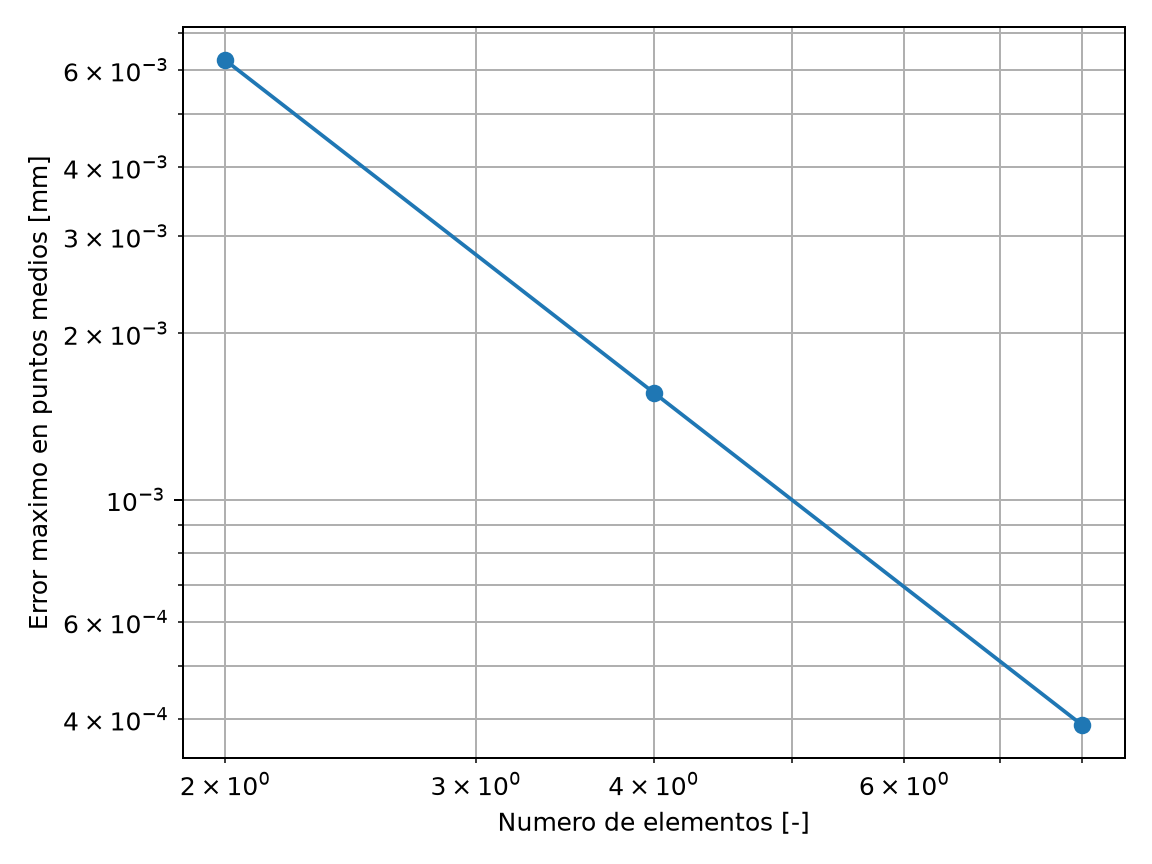
\includegraphics[width=0.65\textwidth]{convergencia.png}
\caption{Convergencia del error absoluto máximo en puntos medios frente al número de elementos $n$ (escala log-log).}
\label{fig:convergencia}
\end{figure}

Se verifica que el balance axial en los tres casos de refinamiento satisface $|R_{\text{izq}} + P + qL| / |P + qL| \le 10^{-8}$, cumpliendo la tolerancia de cálculo impuesta. Las pequeñas diferencias numéricas en M4 y M8 ($\sim 10^{-11}$) responden a precisión flotante de 64 bits.

\section{Interpretación y conclusiones}
El refinamiento de malla ($n=2 \to 4 \to 8$) mantiene exactos el desplazamiento nodal $u(L) = \SI{0.300}{\mm}$ y la reacción $R_{\text{izq}} = \SI{-40000}{\N}$ debido a la convergencia nodal en elementos bajo vectores de carga consistentes. No obstante, el error entre nodos decrece cuadráticamente, dividiéndose por cuatro en cada refinamiento ($e_2 = 0.00625 \to e_4 = 0.00156 \to e_8 = 0.00039\text{ mm}$). Por otra parte, la restricción $u(L)=0$ en \texttt{BC\_ALTERADO} satisface el equilibrio algebraico ($\sum F = 0$), pero altera el problema físico a una barra hiperestática doblemente empotrada, generando una reacción $R_{\text{der}} = \SI{-30000}{\N}$. En conclusión, el cumplimiento del equilibrio prueba que el solver resolvió correctamente el sistema algebraico, pero no garantiza la validez del modelo si las condiciones de contorno han sido mal especificadas.

\section*{Declaración de uso de IA}
Se utilizó asistencia generativa de inteligencia artificial para la derivación simbólica de la solución analítica $u_{\text{ref}}(x)$, la implementación del cálculo de error internodal en \texttt{src/analisis.py} y la elaboraciín de la tabla de datos en LaTeX. Todos los códigos fueron ejecutados localmente, las pruebas unitarias fueron verificadas con \texttt{pytest} y los resultados numéricos fueron contrastados manualmente con la formulación analítica de elementos finitos.

\begin{thebibliography}{9}
\bibitem{guzman_u3l1}
Guzmán, C. F. (2024). \emph{Del problema físico al modelo y al MEF}. Apuntes de clase, Unidad 3: Modelación computacional, Herramientas Computacionales para Ingeniería II, Departamento de Ingeniería en Obras Civiles, Universidad de Santiago de Chile.

\bibitem{guzman_u3l2}
Guzmán, C. F. (2024). \emph{Sensibilidad a malla y condiciones de borde}. Apuntes de clase, Unidad 3: Modelación computacional, Herramientas Computacionales para Ingeniería II, Departamento de Ingeniería en Obras Civiles, Universidad de Santiago de Chile.

\end{thebibliography}

\end{document}